\chapter{System architecture}
The library is based on the client-server architectural pattern and is indeed split in two main modules: 
\begin{itemize}
	\item[Client module] Provide the main functionalities to connect and communicate with a game server. In particular allows the client side developer to create rooms (that will be hosted on the server) and to perform operations on them (e.g join, leave, message...).
	\item[Server module] Internally implements the logic to handle client connections and allows the developer to run a gameserver and define new type of rooms.
\end{itemize}

Cient and server however are not fully separated; they share some common concepts among which the most important, as emerged from the requirements, is the concept of Room.

\section{Room}
As showed in the figure, a room, at the most abstract level, has a unique id and some shared properties. This fields are visible both on the client and the server. Then each module extends his own concept of room. 

\bigskip
\textit{ServerRoom}
\\
The server room is the one that will be used by the server side developer. It aggregates a list of client and provides the main methods to communicate with them (i.e. tell and broadcast).  This component is meant to be abstract so that the user can extend it and define his own behavior (as expressed in requirement 2.1 of table \ref{table:server-f-req})). Since the developer may want to automatically synchronize the state of the game and have an inner game loop (requirements 2.1.2.1 and 2.1.2.2) ther are two extension of the server room: SynchronizedState and GameLoop that provide this functionalities.

\bigskip
\textit{ClientRoom}
\\
This is, on the other hand, the room that a client side developer will use. The user can retrieve a list of JoinableRoom from the server; these expose the method \textit{join} that sends a request to the game server to join the given room; a JoinableRoom can also be used to reconnect to a previously left room as express in requirement 5 of Table \ref{table:client-f-req}. Once the joining process to a room succedes, a JoinedRoom is created and the user can use it to perform operation on the room (requirements 4, 7, 8 of table \ref{table:client-f-req} ) 

\section{Server architecture}
The main components of the server side architecture are visible in figure \ref{fig:server_classes}. 

\begin{figure}[H]
	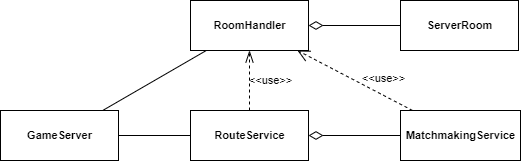
\includegraphics[scale=0.7]{images/3-architecture/server_architecture-classes.png}
	\caption{Server components class diagram}
	\label{fig:server_classes}
\end{figure}

\bigskip
\textit{GameServer}
\\
The GameServer is a facade component that is exposed to the server side developer and provides the functionalities to start and terminate a gameserver; define new type of rooms; create public rooms. To do so, it internally creates two other components that are the RouteService and the RoomHandler.

\bigskip
\textit{RouteService}
\\
The RouteService defines the routes that the server will listen on and implements all the handlers associated with them. The basic routes that the server uses are defined by the following REST protocol 

\begin{itemize}
	\item[GET]  /rooms/:id
	\item[POST] /rooms/
	...
\end{itemize}

Since most of them require to perform operation on rooms (get rooms, create rooms ...),a RoomHandler is used to handle them.

The RouteService has also a list of MatchmakingSystems that are used to handle requests on matchmaking. Each MatchmakingSystem implements the logic expressed in section \ref{server-requirements-gathering}. 

\bigskip
\textit{RoomHandler}
\\
As the name suggests, the RoomHandler is the handler of the rooms in the application. The purpose of this componenet is to provide functionalities regarding rooms, in particular:
\begin{itemize}
	\item get the list of rooms
	\item define new type of rooms
	\item create rooms
	\item query rooms by their properties
\end{itemize}




\section{Client Architecture}

\section{Client-Server Interaction}